The goal of this project was not only to automate the processing of the ULTRACAM raw data, but also to provide a mechanism whereby the entire data archive could be made available for easy access to researchers worldwide. The obvious approach is to make the output of the project available through a web enabled interface. From the outset of the project, all efforts have been focused on ensuring that the resulting data is all accessible through an easy-to-use web interface. 

\section{Web browsers}
In order to make access as easy as possible, a very obvious request is to create a solution that does \emph{not} require the user to install any additional software on their own computer. Since we can reasonably safely assume that everyone who has an interest in accessing the ULTRACAM data has a standard Web browser installed, a web version of this data archive is the best solution. 

A more specific definition of our assumption is that we expect that the user accessing the archive will have a browser that has the capability of rendering HTML5 markup, Javascript and CSS. These technologies are standard in all popular web browsers in mid-2014. The only notable exception is that Internet Explorer, by Microsoft, is not supported in this project. Although Internet Explorer is a modern browser and does have support for the required technologies, its implementation of these technologies is significantly different to that of all of the other browsers and would have required extra coding for support. We felt that, since the majority of astronomers don't use the Microsoft operating system, we were well justified in making this omission.  

\section{Web technologies}
HTML, CSS and JavaScript are three core technologies driving the development of the dynamic, interactive and flexible applications we are becoming accustomed to on the web these days. We chose these three technologies to present the ULTRACAM archive. The result of this is that this archive is immediately available to anyone with a modern web browser and working on any type of computer (desktop, laptop or tablet). There are some high demands on memory, so it is not recommended that the archive is browsed using a mobile phone, although, in theory, there is no functionality that restricts use on such a device (just the memory constraints). 

\emph{HTML} provides the underlying structure of a modern webpage. It is a semantic markup language, meaning that its purpose is to inform the browser on the document's structure. Despite the habit of many people who dabble at making web pages, HTML is \emph{not} meant to be used to alter the presentation of content. \emph{CSS (or Cascading Style Sheets)} is the layer that is meant to inform the browser on how the presentation of each element on the page should look. For example, it might define the fonts or colours for each particular element (or set of elements), like headings, paragraphs, etc. \emph{Javascript} provides the interactive portion of the page, allowing the user to trigger actions when a mouse is clicked or a new object is loaded. It can be used to manipulate the structure of the existing page. It also provides the mechanism for mathematical computation.

Another way of stating this is to say that HTML provides the Semantic structure, CSS the Presentation layer and JavaScript the Programmatic environment. This is also described as the classic "Model-View-Controller" approach used in many development paradigms in the field of Computer Science.

The final stage in the ULTRACAM automated pipeline produces a set of files that are available to a web browser. These files are hosted on a web server that is operated by the University of Warwick CSC team. The pipeline prepares that files and then writes them to the appropriate location in the University's local storage. As soon as the pipeline has finished running, the web pages can be viewed globally. 

\label{sect:clientserver}
Web applications like this, are often refered to as 'client-server' applications, meaning that the application consist of two parts, one running on the client (web browser) and the other running on the server of the institution hosting the application. Obviously, there is a one-to-many relationship between clients and server. There is usually only one server involved, but many clients can connect to that server and interact individually with the application. When writing the web interface for this project we had to make a decision on how much of the functionality we should place on the server versus the client. There were two main, competing, factors to consider:

\begin{itemize}
  \item \emph{Complexity of the application:} Writing an application that has complex components on both the server-side and the client-side, increases the difficulty in launching and maintaining the application. We need to install and configure a web server that is able to run code locally and that also needs access to local data sources, such as databases. If we structure our application such this is only relies on the web server to host and serve static files, then the management of the server-side portion is trivial. If, on the other hand, we decide to split the application code to run on both the client and the server, then we need code on both components in order to coordinate the interaction between the two. Also, the connection between client and server can add some latency (time-lag) to the interactions. This would be noticeable if, say, every time the user clicks on a new object in the field, we need to make a request to the server to fetch a new batch of data to render.  

  \item \emph{Browser memory constraints:} Loading all of the data required to display the results of one of the ULTRACAM runs can be quite demanding on the browser. For some runs there are several hundred objects each with several hundred exposures. This can result in a JSON file for the object data that is \textgreater 1 MByte in size. All of this has to be loaded into the browser's memory. If the user is working on a tablet or an older desktop PC or laptop, then this can cause memory issues. Some long runs with extremely high cadences have very few objects, but hundreds of thousands of exposures and these will tax the memory management of the browser. That said, it is true that for the vast majority of the runs, the memory load on the browser, although significant, is not a problem. 
\end{itemize}

In order to aid rapid development of this project, we decided to opt for a purely client-side code implementation, leaving the web server to serve only static files. This is working adequately in terms of meeting the needs and scope of the project, but it is clear that, for future iterations of this pipeline we should carefully consider moving to an application model that relies more heavily on the server to manipulate, store and serve data. We cannot place any more load on the client. 

As our data storage tool, we chose JSON (JavaScript Object Notation) \footnote{\url{http://json.org/}} as the format as this meant that it could be easily loaded by the Javascript code running in the browser. JavaScript has several built-in methods to load and parse a JSON object. JSON is a flexible, open format that allows a hierarchical structure to be defined for each object stored. It is also designed to be human-readable, meaning that it is possible to open in a text editor and check to contents. The problem with this format is that it is stored as 'plain text' and uncompressed. Also the text format itself defines the structure of each objects it contains, leading to some amount of redundancy in the file (eg the repeating of labels, etc). While it is true that JSON is inefficient in many ways, it is a useful format to use thanks to its flexibility and the ease with which the developer can check and debug the data. 

Many client-server applications use a relational database to store their data, often something like \emph{MySQL}. Since we were not writing any code to run on the server-side and purely relying on the web server for static files, this did not seem appropriate. It is a topic that will be re-considered when we look at implementing server-side code in future iterations of this automated pipeline. 

\section{The Web site}
The core `visible product' of the project is a website that allows a user to browse all of the data in the ULTRACAM archive. The key features of this website are:

\begin{itemize}
	\item A catalog of runs organised by calendar date, containing \emph{thumbnail images} of the fields.
	\item For each run, a web page that shows the user:
	\begin{itemize}
		\item \emph{deep images} of the field in each of the three channels (r, g, b).
		\item \emph{light-curves} of each object as the user clicks on the object with the mouse. 
		\item plots of the \emph{pixel position} of each object over the course of the run.
		\item \emph{world coordinates} of each object, provided that a correct astrometric solution has been found for the run. 
		\item \emph{light curve} for the object that is currently being used as the 'comparison' object. 
	\end{itemize}
	\item light-curves can be plotted as absolute measured flux or a \emph{relative flux} compared to the comparison object in the field. 
	\item the web page allows the user to \emph{export} the data in a CSV format.
	
\end{itemize}
See Fig. \ref{browser} for an example of the web-page. 

\begin{figure}[!h]
	\centering
	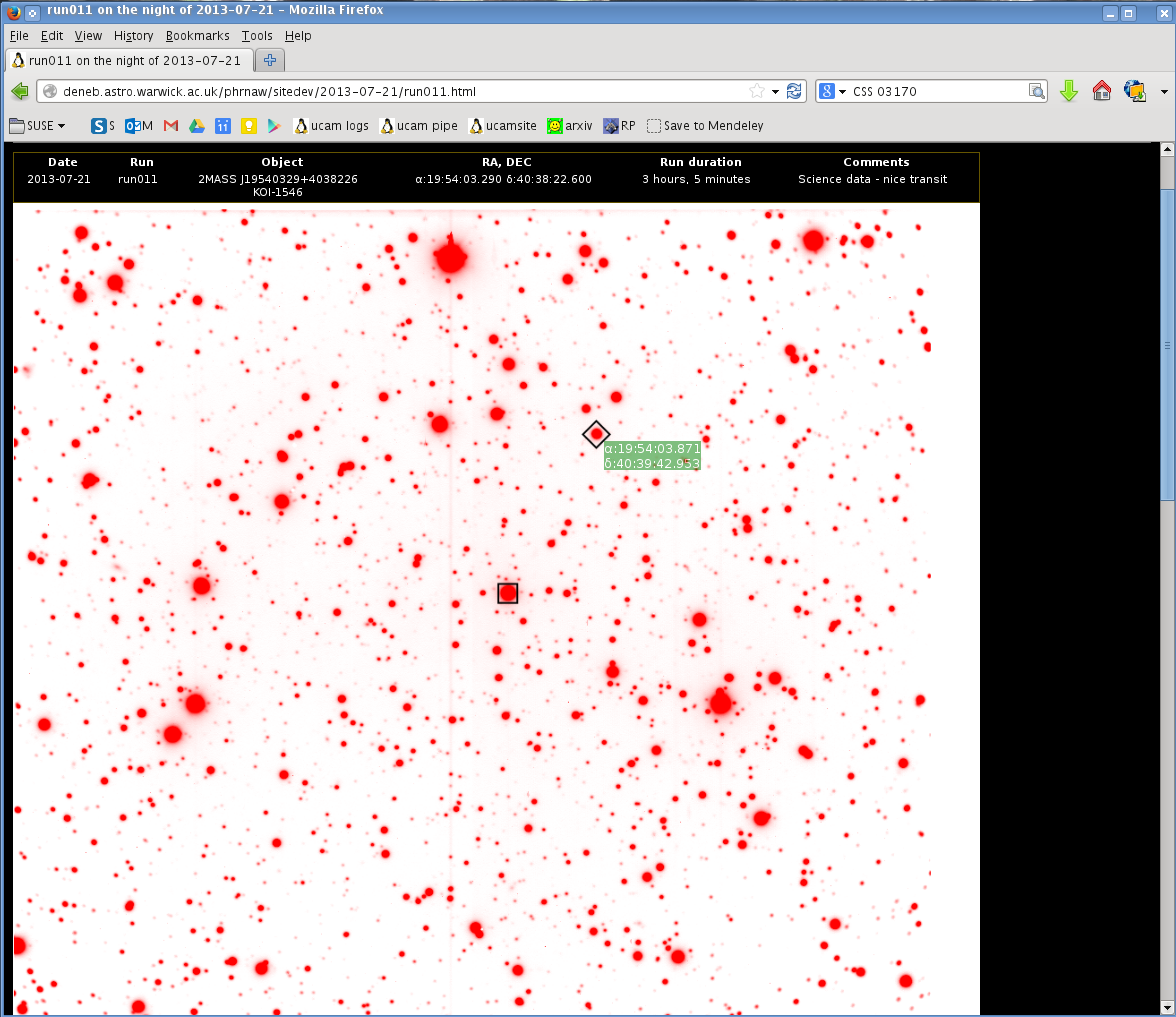
\includegraphics[width=90mm]{images/website1.png}
	\caption{Example of the webpage for browsing the light-curves of a particular run.}
	\label{browser}
\end{figure}

  
\section{Accessing the data}
The pipeline deposits the output HTML, Javascript, image (PNG) and data files (JSON) to a folder that is configured to be server by the University of Warwick's CSC web server at \url{http://deneb.astro.warwick.ac.uk}. Please refer to the User manual to find out how to access and browse the data \ref{chap:usermanual}. 

